\documentclass[12pt, twoside]{article}
\usepackage[letterpaper, margin=1in, headsep=0.5in]{geometry}
\usepackage[english]{babel}
\usepackage[utf8]{inputenc}
\usepackage{amsmath}
\usepackage{amsfonts}
\usepackage{amssymb}
\usepackage{tikz}
\usepackage{yhmath}
%\usetikzlibrary{quotes, angles}

\usepackage{graphicx}
\usepackage{enumitem}
\usepackage{multicol}

\usepackage{fancyhdr}
\pagestyle{fancy}
\fancyhf{}
\renewcommand{\headrulewidth}{0pt} % disable the underline of the header

\fancyhead[R]{\thepage}
\fancyhead[L]{BECA / Dr. Huson / 10th Grade Geometry\\* Learning trajectory: Area, perimeter, volume}

\begin{document}
\subsubsection*{Area, perimeter, volume}
  \begin{enumerate}
    \item Prior knowledge
      \begin{enumerate}
        \item Area: rectangle, square, triangle, parallelogram; area and perimeter (formula sheet)
        \item Solve for parameter versus calculate result
      \end{enumerate}

    \item Distance on the coordinate plane
      \begin{enumerate}
        \item Plotting, labeling points, etc.
        \item Horizontal \& vertical distances
        \item Perimeter calculation
        \item Pythagorean formula
        \item Applications: Rhombus, isosceles $\triangle$,
        \item Radicals, $\pi$ and rounding
      \end{enumerate}

    \item Volume: prism, cylinder, cone
      \begin{enumerate}
        \item Compound shapes (including margins)
        \item Surface area
      \end{enumerate}

    \item Circle area and circumference
      \begin{enumerate}
        \item Sector areas, arc length
        \item Radian / degree conversion
      \end{enumerate}

    \item Scaling shapes (eg. rectangle, triangles including midline)

    \item Regents problems, January 2017, \#26, 34, 29? (basic shapes)
  \end{enumerate}

\newpage
\subsubsection*{Horizontal and vertical measure}
\begin{enumerate}

  \item Given the quadrilateral $ABCD$ with $A(1,2)$, $B(6,2)$, $C(6,5)$, and $D(1,5)$.
    \begin{enumerate}
      \item Plot and label $ABCD$ on the grid.
      \item Find the lengths of the sides by counting on the graph or subtracting coordinates. Complete the table.
      \item Definition: Perimeter is the total distance around a shape.\\[0.25cm]
      Add up the perimeter of $ABCD$, entering it to the bottom of the table of lengths.\\
        \begin{multicols}{2}
          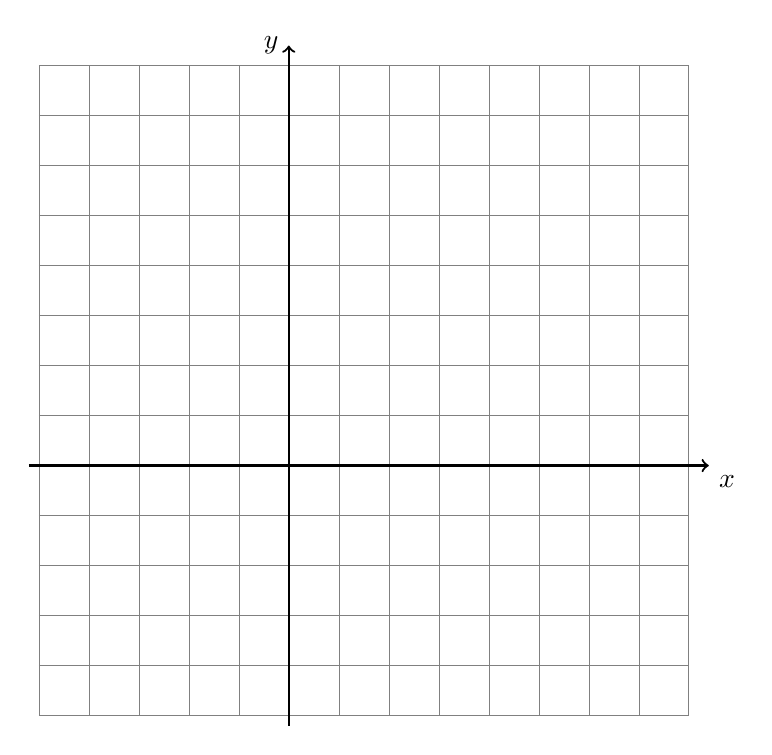
\begin{tikzpicture}[scale=.635]
            \draw [help lines] (-5,-5) grid (8,8);
            \draw [thick, ->] (-5.2,0) -- (8.4,0) node [below right] {$x$};
            \draw [thick, ->] (0,-5.2)--(0,8.4) node [left] {$y$};
          \end{tikzpicture}\\
          \renewcommand{\arraystretch}{1.5}
          \begin{flushright}
          \begin{tabular}{|p{1cm}|p{2cm}|}
            \hline
            Side & Length \\
            \hline
            $AB$ & \\
            \hline
            $BC$ & \\
            \hline
            $CD$ & \\
            \hline
            $AD$ & \\
            \hline
            Total & \\
            \hline
          \end{tabular}
        \end{flushright}
        \end{multicols}
      \item Definition: Area is the number of unit squares in a shape. \\[0.25cm]
      Find its area by counting the number of squares in $ABCD$ or use multiplication as a short cut.
    \end{enumerate}

\newpage
  \item The rectangle $ABCD$ is shown below with length $l=12$ and width $w=5$. Label the sides of the rectangle with their lengths.
  \begin{enumerate}
    \item Calculate the perimeter and enter it in the table.
    \item Find the area of the rectangle. (show the work as an algebra equation)
    \begin{multicols}{2}
      \begin{tikzpicture}[scale=.635]
        \draw [thick] (0,0)node[below]{$A$}--
        (12,0)node[below]{$B$}--
        (12,5)node[above]{$C$}--
        (0,5)node[above]{$D$}--cycle;
      \end{tikzpicture}\\
      \renewcommand{\arraystretch}{1.5}
      \begin{flushright}
      \begin{tabular}{|p{2cm}|p{2cm}|}
        \hline
        Side & Length \\
        \hline \hline
        $AB$ & 12 \\
        \hline
        $BC$ & 5 \\
        \hline
        $CD$ & 12 \\
        \hline
        $AD$ & 5 \\
        \hline \hline
        Perimeter & \\
        \hline
      \end{tabular}
    \end{flushright}
    \end{multicols}
  \end{enumerate} \vspace{1cm}

  \item Given the quadrilateral $BECA$ with $B(-3,-2)$, $E(5,-2)$, $C(5,5)$, and $A(-3,5)$.
    \begin{enumerate}
      \item Plot and label $BECA$ on the grid.
      \item Find the lengths of the sides and complete the table.
      \item Calculate the perimeter and enter it in the table.\\
        \begin{multicols}{2}
          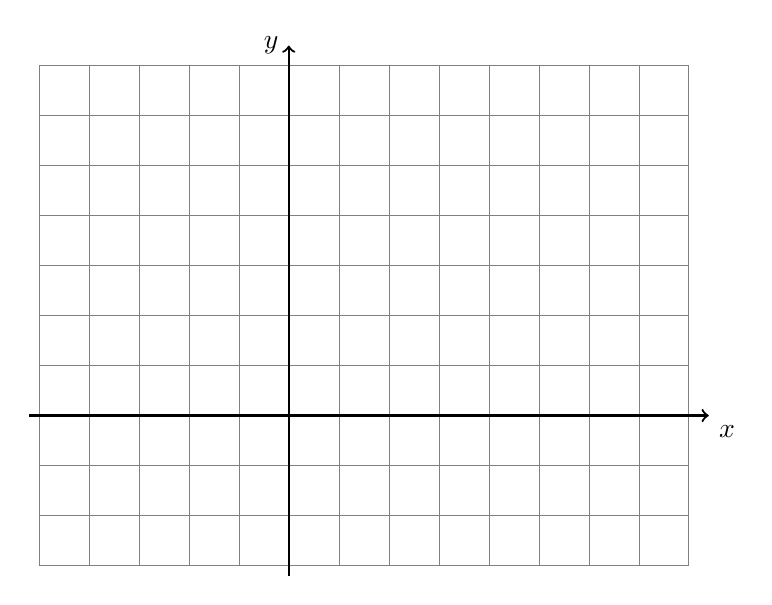
\begin{tikzpicture}[scale=.635]
            \draw [help lines] (-5,-3) grid (8,7);
            \draw [thick, ->] (-5.2,0) -- (8.4,0) node [below right] {$x$};
            \draw [thick, ->] (0,-3.2)--(0,7.4) node [left] {$y$};
          \end{tikzpicture}\\
          \renewcommand{\arraystretch}{1.5}
          \begin{flushright}
          \begin{tabular}{|p{1cm}|p{2cm}|}
            \hline
            Side & Length \\
            \hline
            $BE$ & \\
            \hline
            $EC$ & \\
            \hline
            $CA$ & \\
            \hline
            $AB$ & \\
            \hline
            Total & \\
            \hline
          \end{tabular}
        \end{flushright}
        \end{multicols}
      \item Find the area of $BECA$.
    \end{enumerate}

\newpage
  \subsubsection*{Diagonal distance on the coordinate plane}
  \item Given $P(-2,9)$ and $Q(3,-3)$, find the length of $\overline{PQ}$.

  \subsubsection*{Distance on the coordinate plane: proofs}

    \item Triangle $ABC$ has vertices with coordinates A(,), B(,), and C(,). Prove that $\triangle ABC$ is an isoscelese triangle but not an equilateral triangle. (The use of the set of axes below is optional.)\\
    Note: state both conclusions for full credit.

    \item Triangle $\triangle TEN$ is graphed on the set of axes below. The vertices of $\triangle TEN$ have the coordinates $T(-1,-2)$, $E(8,1)$, and $N(3,6)$.
      \begin{center} %4 quadrant regents grid
      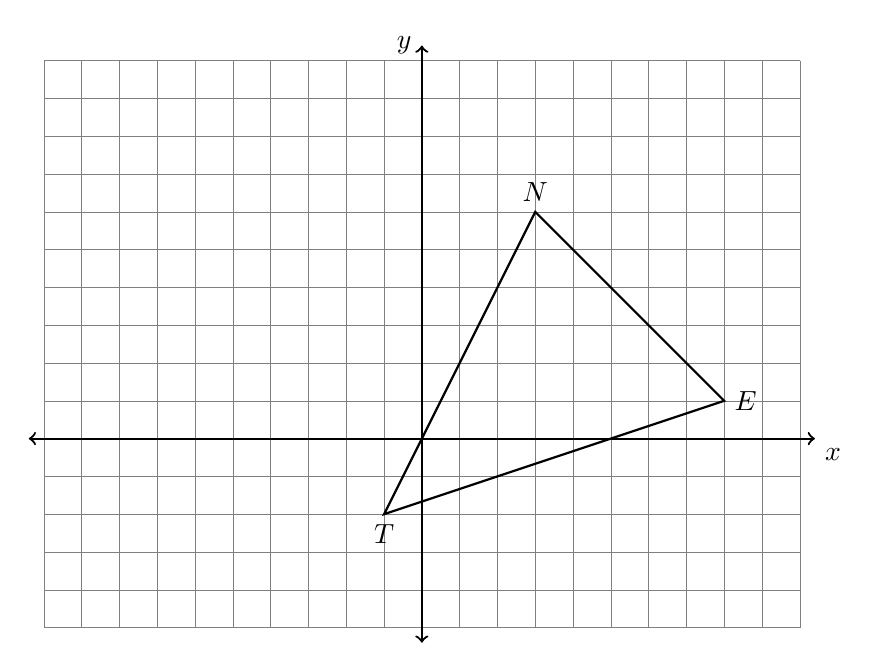
\begin{tikzpicture}[scale=.48]
        \draw [help lines] (-10,-5) grid (10,10);
        \draw [thick, <->] (-10.4,0) -- (10.4,0) node [below right] {$x$};
        \draw [thick, <->] (0,-5.4)--(0,10.4) node [left] {$y$};
        \draw [thick]
          (-1,-2) node[below] {$T$}--
          (8,1) node[right] {$E$}--
          (3,6) node[above] {$N$}--cycle;
      \end{tikzpicture}
      \end{center}
      \begin{enumerate}
        \item Draw an altitude through point $N$ perpendicular to $\overline{TE}$.
        \item What is the length of the altitude drawn through $N$?
        \item What is the length of the base, $TE$?
        \item Find the area of  $\triangle TEN$.
      \end{enumerate}

      \item Given the quadrilateral $RSTU$ with $R(1,3)$, $S(4,7)$, $T(4,2)$, and $U(1,-2)$.
        \begin{enumerate}
          \item Plot and label $RSTU$ on the grid.
          \item Using the distance formula or otherwise, calculate $RS$, $ST$, $TU$, and $RU$.
          \item Definition: If a quadrilateral has four congruent sides, then it is a rhombus.\\[0.5cm]
          Prove that $RSTU$ is a rhombus.
        \end{enumerate}
        \begin{center} %4 quadrant regents grid
        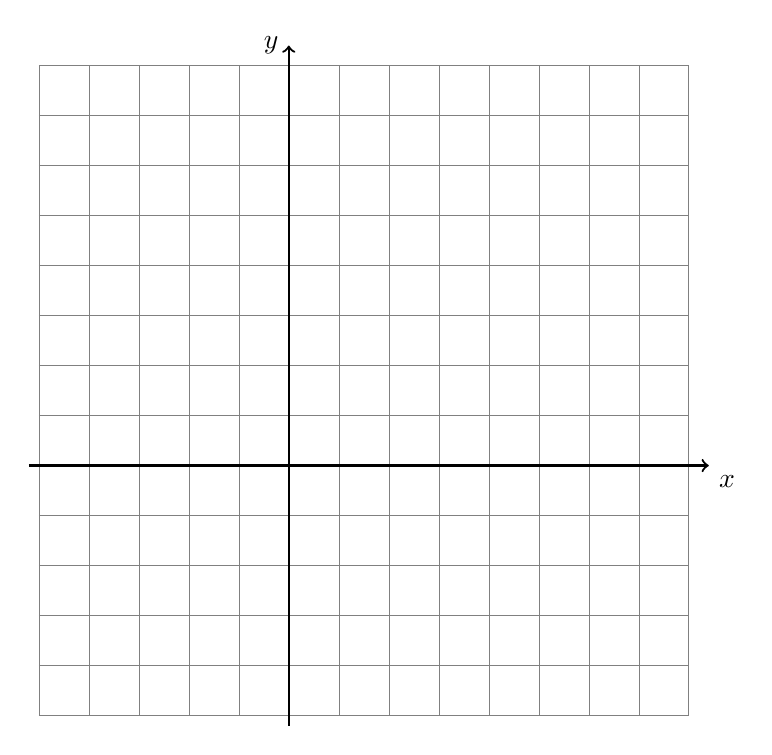
\begin{tikzpicture}[scale=.635]
          \draw [help lines] (-5,-5) grid (8,8);
          \draw [thick, ->] (-5.2,0) -- (8.4,0) node [below right] {$x$};
          \draw [thick, ->] (0,-5.2)--(0,8.4) node [left] {$y$};
        \end{tikzpicture}
        \end{center}

    \item Given the quadrilateral $RECT$ with $R(-4,1)$, $E(8,1)$, $C(8,6)$, and $T(-4,6)$.
      \begin{enumerate}
        \item Plot and label $RECT$ on the grid.
        \item Using the distance formula, calculate the length of the two diagonals $RC$ and $ET$.
        \item Theorem: If the diagonals of a quadrilateral are congruent, then it is a rectangle.\\[0.5cm]
        Prove that $RECT$ is a rectangle.
      \end{enumerate}
      \begin{center} %4 quadrant regents grid
      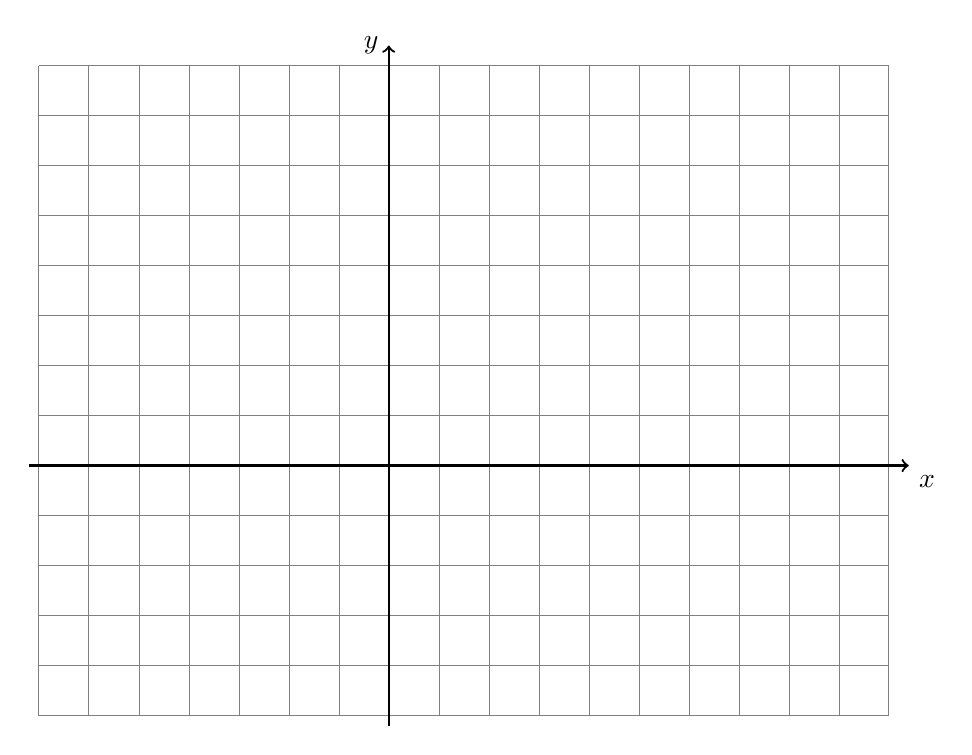
\begin{tikzpicture}[scale=.635]
        \draw [help lines] (-7,-5) grid (10,8);
        \draw [thick, ->] (-7.2,0) -- (10.4,0) node [below right] {$x$};
        \draw [thick, ->] (0,-5.2)--(0,8.4) node [left] {$y$};
      \end{tikzpicture}
      \end{center}

    \subsubsection*{Circle area and circumference}
      \item %June 2018
      The diagram below shows the circle $O$ with radii $\overline{OA}$ and $\overline{OB}$. The measure of angle $AOB$ is $120^\circ$, and the length of a radius is 6 inches.
      \begin{center}
      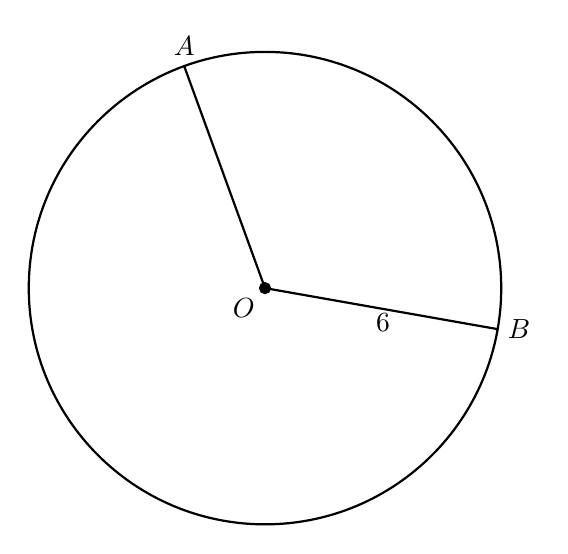
\begin{tikzpicture}
        \draw [thick] (0,0) circle[radius=3cm];
        \draw [thick, -]
          (110:3)node[above]{$A$} --
          (0,0) node [below left]{$O$}--
          (-10:3)node[right]{$B$};
          \draw [fill] (0,0) circle [radius=0.07];
        \node at (1.5,-0.2)[below] {6};
      \end{tikzpicture}
      \end{center}
      Which expression represents the length of arc $AB$, in inches?
      \begin{multicols}{2}
        \begin{enumerate}
          \item $\displaystyle \frac{120}{360}(6\pi)$
          \item $120(6)$
          \item $\displaystyle \frac{1}{3}(36\pi)$
          \item $\displaystyle \frac{1}{3}(12\pi)$
        \end{enumerate}
    \end{multicols}
    %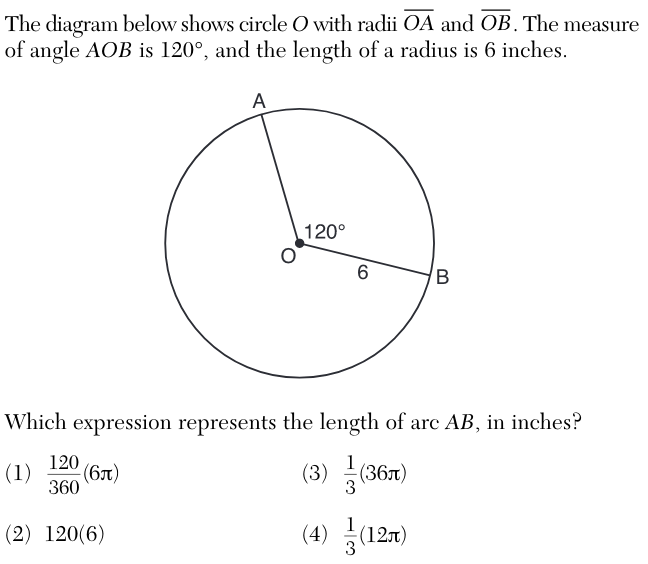
\includegraphics[width=0.85\textwidth]{Circle_JN2018-22.png}

    \item %August 2019
    Circle O with a radius of 9 is drawn below. The measure of central angle AOC is $120^\circ$.
    \begin{center}
      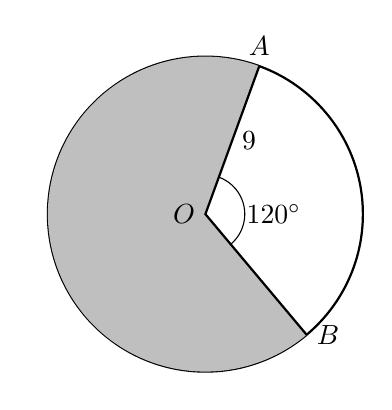
\begin{tikzpicture}
        \draw [thick] (0,0) circle[radius=2cm];
        \fill [lightgray] (-50:2)--(0,0)--(70:2)arc(70:310:2);        \draw [thick, -]
          (70:2)node[above]{$A$} --
          (0,0) node [ left]{$O$}--
          (-50:2)node[right]{$B$};
        \node at (70:1)[right]{9};
        \node at (0:0.4)[right]{$120^\circ$};
        \draw (-50:0.5) arc(-50:70:0.5);
      \end{tikzpicture}
      \end{center}
    What is the area of the shaded sector of circle $O$? 
      \begin{multicols}{2}
        \begin{enumerate}
        \item $6\pi$
        \item $12\pi$
        \item $27\pi$
        \item $54\pi$
      \end{enumerate}
    \end{multicols}

  \item %June 2019
  In the diagram below, circle O has a radius of 10.
  \begin{center}
    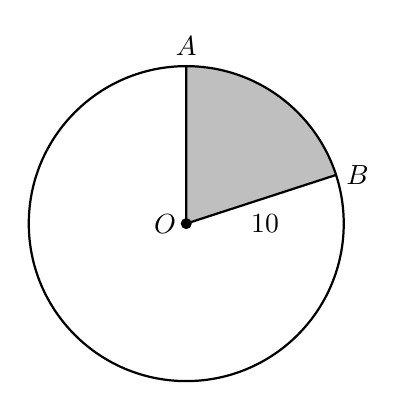
\begin{tikzpicture}
      \fill [lightgray] (90:2)--(0,0)--(18:2)arc(18:90:2);
      \draw [thick] (0,0) circle[radius=2cm];
      \fill (0,0) circle[radius=0.07];
      \draw [thick, -]
        (90:2)node[above]{$A$} --
        (0,0) node [ left]{$O$}--
        (18:2)node[right]{$B$};
      \node at (0:1){10};
      %\node at (0:0.4)[right]{$120^\circ$};
      %\draw (-50:0.5) arc(-50:70:0.5);
    \end{tikzpicture}
    \end{center}
    If $m \wideparen{AC}=72^\circ$, find the area of shaded sector AOB, in terms of $\pi$.

  \item %January 2018
  In the diagram below, the circle has a radius of 25 inches. The area of the \emph{unshaded} sector is $500\pi$ $\mathrm{in}^2$.
  \begin{center}
    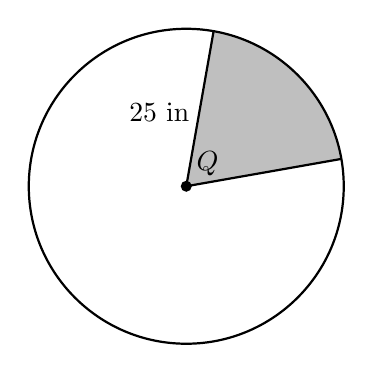
\begin{tikzpicture}
      \fill [lightgray] (80:2)--(0,0)--(10:2)arc(10:80:2);
      \draw [thick] (0,0) circle[radius=2cm];
      \fill (0,0) circle[radius=0.07];
      \draw [thick, -] (80:2)--(0,0) node [above right]{$Q$}--(10:2);
      \node at (110:1){25 in};
    \end{tikzpicture}
    \end{center}
    Determine and state the degree measure of angle $Q$, the central angle of the shaded sector. %72 degrees
    
  \item %January 2019
  The area of a sector of a circle with a radius measuring 15 cm is $75\pi$ $\mathrm{cm}^2$. What is the measure of the central angle that forms the sector?
    \begin{multicols}{2}
      \begin{enumerate}
      \item $72^\circ$
      \item $120^\circ$
      \item $144^\circ$
      \item $180^\circ$
    \end{enumerate}
  \end{multicols}

  \item %August 2018
  A circle with a diameter of 10 cm and a central angle of $30^\circ$ is drawn below.
  \begin{center}
    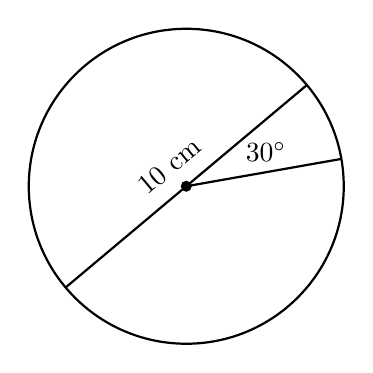
\begin{tikzpicture}
      \draw [thick] (0,0) circle[radius=2cm];
      \fill (0,0) circle[radius=0.07];
      \draw [thick, -](220:2)--(0,0)--(40:2);
      \draw [thick, -](0,0)--(10:2);
      \node at (23:1.1){$30^\circ$};
      \node at (130:0.1)[above, rotate=40]{10 cm};
      %\draw (-50:0.5) arc(-50:70:0.5);
    \end{tikzpicture}
    \end{center}
  What is the area, to the \emph{nearest tenth of a square centimeter}, of the sector formed by the $30^\circ$ angle?
    \begin{multicols}{2}
      \begin{enumerate}
      \item 5.2
      \item 13.1
      \item 6.5
      \item 26.2
    \end{enumerate}
    \end{multicols}
    

    
  \end{enumerate}
\end{document}
